\chapter{Design and Implementation}

\todo{Assigned Johan L}

This chapter describes the design and implementation of the Hopper language and its compiler with all the compiler components. There will be overviews of each part describing the choices made and the reasoning behind those choices.

%The chapter starts with the design of the language and how it affected the ensuing work on the compiler.
%The initial design of Hopper included choices affecting the implementation of the compiler. 

\todo{Brief dscription of the grammar, features, maybe misc topics of interest that dont have any immediate section to be written in}

When first designing Hopper there was already an outline of what the language should aim to be. The type safety and clean syntax of Haskell combined with the powerful framework for concurrency and parallelism supplied by the Erlang virtual machine was the key words from which Hopper would be built. Within those confines there were further choices as to what features to include, and not to include, to make the language relevant and useful.

Features.

Discuss the most relevant features here...

Grammar.

\todo{Talk about grammar here or in D&I: Parser?}

\todo{delete D&I: the hopper language}

%\section{The Hopper language}

\todo{Assigned Johan L}

\todo{move to intruduction of chapter 4}

\todo{Brief dscription of the grammar, features, maybe misc topics of interest that dont have any immidiate section to be written in}

\section{The compiler pipeline}

% PIPELINE FIGURE

\begin{figure}[h!]
\centering
  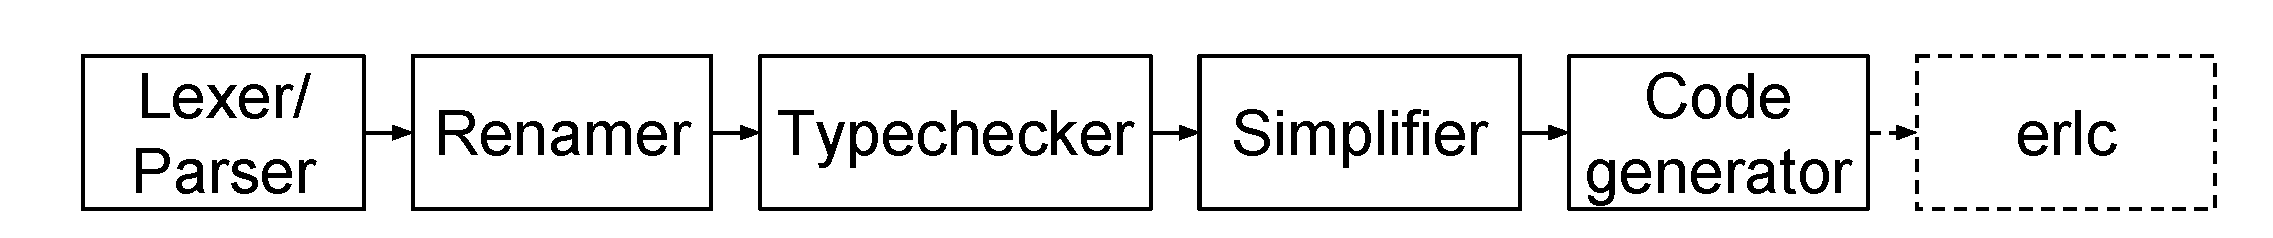
\includegraphics[width=0.6\pdfpagewidth]{figure/pipeline}
  \caption{Hopper's pipeline}
  \label{fig:pipeline}
\end{figure}

% HOW IS HOPPER BUILT

As seen in figure~\ref{fig:pipeline} the Hopper language has five steps in its compiler
pipeline before it turns over to the Erlang compiler. Each step works on the 
source code representation in a uniqe way. The steps can be summerized as
follows. The lexer and parser reads in text files and converts them to an 
abstract representation, the renamer then simplifies this representation for the 
type checker whose job it is to control the types of all the expressions. Lastly 
there is another simplifying step before the code generator which produces Core
Erlang code. The Erlang compiler is then invoked, using the produced Core Erlang
code, and the result is Erlang assembly code that is run on the BEAM VM.

\section{Parser}

\todo{Assigned to David}

%\todo{Reduce the number of subsections}
%\todo{Write more about grammar, have grammar in appendix}

The parser is implemented by a BNF grammar that is converted to a lexer and 
parser with the BNFC tool. 

%\subsection{BNFC - automatic generation}

BNFC, as described in the background, is the Backus Naur Form Converter developed at Chalmers which the group used to automatically generate a lexer and parser. The group had to write a grammar for the Hopper language in Backus Naur Form and feed it to BNFC which then, for Haskell, uses Alex and Happy to produce the lexer and parser.

Starting the project there were discussions in the group on whether or not to use BNFC to generate the lexer and parser. Choosing to get an easy start with the generated lexer and parser was accompanied by the notion that the group might want to switch to using Alex and Happy directly at a later stage. This did not come to happen during the project but might still be something to consider for the future. Implementing the groups own lexer and parser would mean greater control over the process.
\todo{does this discussion belong in background (or dicussion) instead? fill out}

\todo{talk about layout, inserting of \{ and ; }

\subsection{The grammar}

Writing the grammar one, in effect, describe the ways in which programs accepted in the language can be written. Hence it takes great consideration to detail to ensure that the grammar allows everything that the language is supposed to be able to express but disallows everything else. This doesn't include expressions that are semantically wrong. For this, semantic analysis of the \acrshort{ast} has to be done with a, for example, type checker. 

The grammar was produced incrementally in steps that allowed more and more syntax to be added. This made it possible to have new functionallity implemented through the whole pipeline before new syntax was added. 

A full rewrite of the grammar was done half way through the project. The reson for this was that some grammatical rules was intertwined and understanding had been improved how a grammar should be defined more correct. The new grammar was more modular which also made the futher extensions simpler.

The final grammar for the language supports most of the necessary syntax for a pure functional programming language. The main features are:

\begin{itemize}
  \item Function definitions and type signatures
  \item Abstract data types
  \item Lambda and case expressions
  \item Patter matching
  \item Module definitions with imports and exports
\end{itemize}


Some syntactic sugar for \texttt{if-then-else} exists and more was planned but didn't made it to the final release. For example sugar for lists.%and something more?

\todo{Improve choice of words/phrasings} 

\todo{Add refs}


\section{Renamer}

\todo{Assigned David}

The renamer is implemented by traverse the parse tree obtained from the parser. In this traverse the renamer builds up a new tree of constructors for the languge minimally designed \acrshort{ast}. 

In this traverse the renamer have plenty of things to do other than a pure translation to a new data type. Some of the things are:

\begin{enumerate}
  \item Merge function definitions with same name.
  \item Merge type with its function definition.
  \item Convert a \acrshort{adt} defintion to a abstract function type.
  \item Check if a function application is a \acrshort{bif}.
  \item Do a few simplifications (see figure \ref{lst:renamer1}).
\end{enumerate}
\todo{Rewrite in text?}

While implementing the renamer much consideration was done of what later stages of the compilation needed. For example, while Erlang allows pattern matching function Core Erlang does not. This is the reason for merging function definitions to a single definition with a case expression and each previous function as a clause. For the same reason was the type data type changed to fit better with the type checker. 

\Acrlong{adt}s was a big milestone for the project. It was considered one of the big things needed to work to make a functional product. Still is the functionality behind them is very simple. When the renamer encounter an ADT definition it just converts each constructor to a function with just a type, no real definition. With this the type checker can verify it's used correctly and leaving it fully to the code generation to implement it without any dependencies. \todo{Remove? Forward ref to codegen adt?}

\todo{Remove the word "definition" a few times maybe?}
\section{Dependency checker}
\label{sec:dai_depcheck}

\todo{Assigned Jakob}
The dependency model of Hopper is rather simple. Modules explicitly declare what functions and data types they export, and declare dependency
on other modules using \texttt{import} statements. Hierarchical module
names are supported, e.g. \texttt{A.B.C}. Only a single
source directory is supported, so there is a straight-forward map from module
names to file paths: the above example maps to \texttt{A/B/C.hpr}. This
restriction simplifies the work of the dependency checker, by removing the concept of conflicts where multiple matching source files exist in different source directories.

The import statements are used to build a \gls{dag}. Verifying that the graph actually is acyclic ensures that no cyclical dependencies occur. Topologically sorting the nodes of the \gls{dag} gives a compilation order where the dependencies of each module are compiled before that module. This design ensures that type information for a module's dependencies is available at compile time, so that the compiler only has to consider a single module at a time.

In order to propagate type information for a given module's exports into the modules that depend on it, the concept of interface files (similar in concept to those of Haskell's\todo{reference here}) is used. They contain type information (which might have been given explicitly, or inferred by the type checker) for everything that is exported from a given module. The actual implementation of the interface files simply uses derived \texttt{Show} and \texttt{Read} instances for the data types representing Hopper types.

\todo{further explain why this is a good organisation}


\section{Type checker}

\todo{Assigned to Liam}

\subsection{The type system}
Rough draft:
\

\todo{please fix layout in generated pdf, the pdf is barely readable right now}
\todo{remove any old type checker stuff that is not used! if anything is kept it should be worked on to fit with the rest}

What do we do in TC/Convert?\

•	Implement constructors (thus allowing codegen to have no knowledge of types)
•	Give some functions implicit type arguments : abused syntax to achieve this. In some ways more powerful than Haskell’s class system (because it is done at runtime in normal Hopper), but more boilerplatey and performance intensive. Allowing values to vary based on their type (i.e. ad-hoc-polymorphism, where polymorphic values are more than just a black box, see Theorems for Free [reference?]) is essential for implementing typesafe message passing, because type information must be sent in messages at runtime to distinguish between values with same runtime representation but different types (e.g. an empty list of Booleans and an empty list of numbers).
•	Implemented receive: abused syntax using case receive of ... -> ...
•	A module that Converts to/from AST.AST. This is bad and is purely technical debt. Why it was created and maintained (two different ASTs, inertia, poor coordination) can be elaborated on in Discussion.
•	Prim.apply\

What can we do with the type system?\

•	Higher order functions, a lot of that Haskelly goodness.
•	IO, other types which describe processes and the connections between them. Because the BEAM is a high level VM designed for a dynamic programming language, coercing between types in Hopper does not have the same catastrophic consequences as in Haskell (which compiles to native machine code: coercing something on the heap can lead to a fatal crash e.g. because you treat a number as a pointer). That means it is rather comfortable to treat the same value as several different types in Hopper: for example a Number may be both a Natural and a Prime. We do not yet know where that leads, but it seems exciting. 
\
(Here ends the draft I added tonight)
\


Hopper uses the Damas-Hindley-Milner (HM) type system for the lambda calculus. HM has parametric polymorphism enabling (wording, what do I mean and what does this say???) type inference of type schemes - types with generic, quantified type variables. Further HM has the Algorithm W which not only infers the most general type for expressions but also has existing soundess and completeness proofs. These proofs means that for our well formed expressions we will always find a type and that it will be the correct type.

\subsection{Preprocessing}

Damas-Hindley-Milner is a type system for the lambda calculus and the parsed Hopper code has a different representation. The parsed code is transformed into an AST and the expressions written in Hopper is turned into semantically equivalent expressions in the lambda calculus. Hopper type inference is done on a simple language which is lambda calculus extended with let expressions and the fixpoint combinator. Lambda calculus in itself is Church-Turing complete and could thus represent these added constructs but they simplify ... (add stuff here)

\begin{description}
\item[The simple language] \hfill
\begin{description}
  \item[Variables] \hfill \\
    A variable is an expression.\\
    Ex. x is a valid expression.
   \item[Abstraction] \hfill \\
    An abstraction of a variable over some expression. (wording?)\\
    Ex. (\textbackslash x . x) is a valid expression.
   \item[Application] \hfill \\
    An application of an expression to another expression is an expression.\\
    Ex. (f x) is a valid expression.
   \item[Extensions] \hfill
\begin{description}
    \item[Let] \hfill \\
      A let expression, defining a variable within the scope\\
      of an expression, is an expression.\\
      Ex. (let x = n in (f x)) is a valid expression. 
    \item[Fix] \hfill \\
      The fixpoint combinator enables recursive expressions.\\
      A fixpoint combinator y satisfies y f = f (y f).
\end{description}
\end{description}
\end{description}

\subsection{Type inference with Algorithm W}

Where the original Algorithm W uses a top-down approach we have chosen to implement it using a bottom-up approach (sometimes called Algorithm M REF: generalizing hindley-milner type inference algorithms, Heeren,Hage,Swierstra ). The bottom-up approach generates constraints on the types in a first pass and then solves these constraints producing the most general type for each expression.

\begin{description}
  \item[Generating constraints by inference rules] \hfill \\
A first pass generates constraints on the types by a set of inference rules (see appendix). \todo{FILL OUT}
  \item[Solving constraints by solving rules] \hfill \\
Secondly we solve the inferred types using the accumulated constraints to produce the most general type for each expression. \todo{FILL OUT}
\end{description}

\section{Code generator}

Generally the last step of a compiler is the code generation step. The code generator
component should take an \gls{ast} much like one of the target language and translate it
to actual code strings of the target language. Additionally, this component may also
perform some optimizations on the generated code before returning it.

\subsection{Implementation}

The code generator is implemented using the Language.CoreErlang \cite{CoreErlang} package
from Hackage (maybe also bibliography link, or glossory). This package contains a Core Erlang
parser, a data structure used for representing Core Erlang \gls{ast}'s and a pretty printer for
said data structure. The code generator makes use of this package by building Core Erlang
\gls{ast}'s and then simply invoking the pretty printer on them to  produce Core Erlang.

Due to the differences between Hopper and Core Erlang, and the additional type constraints
of the Hopper language, the type checker and the code generator require differently
structured \gls{ast}'s . To deal with this another \gls{ast} transformation step has been added
to the compilation time line before the code generation. This step attempts to seperate variables
and function identifiers from each other, and bind function calls with the tokens that
should be used as parameters in said function calls.

\todo{Subsection about constructor to atom translations, JohanWS/Liam}

\todo{Subsection about function applications and the built in curry function, JohanWS/Liam}

\subsection{Emulating the erlang compiler}

One downside to the choice of compiling to Core Erlang and then invoking the erlc
(bibliography link here) is the loss of the additions and optimizations the erlc
compiler makes when it compiles Erlang to Core Erlang in its pipeline. To deal with this
the code generator has been given additional functionality to emulate the pre Core Erlang
behaviour of the erlc compiler. (Proceed to list features here)
